% EXEMPLE de MATHS
% PDFLATEX permet d'ins�rer des images de format "normal" : Jpg, Png...
%Clic sur bouton "PDFLATEX" pour compiler ce document ;
% clic sur bouton "VOIR PDF", pour le visualiser.

\documentclass[11pt,a4paper]{article}		% Format de page pour "article"
\pagestyle{plain}		% pas pied page donc pas numero page
\usepackage[utf8]{inputenc}			% Pour les caract�res accentu�s
\usepackage[T1]{fontenc}				% Encodage de caract�res
\usepackage{lmodern}					% Police vectorielle Latin Modern
\usepackage[frenchb]{babel}				% R�gles typographiques fran�aises
\usepackage{amsmath,amsfonts,amssymb,mathrsfs}			% Symboles math�matiques
\usepackage{graphicx}					% Ins�rer des images
\usepackage[left=2cm, right=2cm, top=2cm, bottom=2cm]{geometry}	%  marges
\usepackage{array}                % tableaux
\usepackage{multirow}                % tableaux de plusieurs colonnes
\usepackage{multicol}                % plusieurs colonnes dans texte
\usepackage{wrapfig}
\usepackage{booktabs}
\def\changemargin#1#2{\list{}{\rightmargin#2\leftmargin#1}\item[]}
\let\endchangemargin=\endlist   %Permet de chager la taille des marge localement

\usepackage{algorithmic}
\usepackage[ruled]{algorithm2e}

% TRAIT entre COLONNES de textes :
%\setlength{\columnseprule}{1pt}		% trait entre colonnes
\setlength{\columnsep}{20pt}		% largeur de separ entre colnnes
\usepackage{epstopdf}
\setlength{\parskip}{8pt plus2pt minus1pt}   %  saut entre paragraphes
\renewcommand{\labelenumii}{\arabic{enumi}.\arabic{enumii}.}    % listes numerotees imbriquees ex :  2.1.1.4
\renewcommand{\labelenumiii}{\arabic{enumi}.\arabic{enumii}.\arabic{enumiii}}
\renewcommand{\labelenumiv}{\arabic{enumi}.\arabic{enumii}.\arabic{enumiii}.\arabic{enumiv}}
\usepackage{xspace}  % espaces sp�ciaux
\usepackage{graphicx,xcolor}
% commande \EUROS
\newcommand{\euros}{\ensuremath{~\epsilon\xspace}}
\DeclareMathOperator*{\argmin}{arg\, min}
% Chamin d'acc�s images :
\graphicspath{{Images/}}

\newcommand{\hu}{\ensuremath{\hat{u}}}

\newcommand{\e}{\ensuremath{\underline{e}}}
\newcommand{\te}{\ensuremath{\underline{\tilde{e}}}}

\newcommand{\dive}{\ensuremath{\operatorname{div}}}
\newcommand{\grad}{\ensuremath{\operatorname{\underline{grad}}}}

\begin{document}

% TITRE ENCADRE'
\begin{center}
\fbox{ \begin{minipage}{10cm}
\begin{center}
\large\textbf{{Generation of safe lanes}}

\end{center}
\end{minipage} }
\end{center}

In this report, we explain how to implement an algorithm that creates a coherent mesh of safe lanes that protects roads between assets. In this approach, the traffic problem is solved as a linear impedance problem between distant nodes, as it is classically done in economics. The mesh of lane that is generated aims at optimizing some cost-function that aims at measuring how hard it is to travel along the lanes. To perform this, we compute the gradient of this cost-function by the adjoint-state method and at each iteration, the best lane in each system is generated. Even if the solution it converges to is very probably sub-optimal, this algorithm shows good general behaviour and seems to be usable as a safe lane generator.

\section{Introduction}

When seen as a topological optimization problem, the generation of safe lanes needs to be based on a direct path-finding problem. The Dijkstra shortest-path algorithm could seem to be the best choice in that case. However, it suffers from one very penalizing flaw: as far as the author knows, there is no simple way to compute the gradient of the operator with respect to the impedance of the paths \footnote{AFAIK, the shorter-path problem is not even well-posed in sense of Hadamard (because of lack of continuity)}. For that reason, it is preferred to solve the path-finding problem as an impedance problem.

In this context, the computation of the gradients can be done at very low computational cost via the adjoint method, and a gradient-based optimization method can be carried up. However, in the present case, this minimization problem is very susceptible to have many constraints (mostly related to the interaction between lanes of different factions). The constraints will probably cause the cost-function to be not convex with respect to the parameters of the optimization, and cause difficulties to a minimization algorithm. For this reason, it was chosen to use a much simpler algorithm, as described in the abstract, that however is very likely to converge to a sub-optimal solution.

This report is divided as follows: the direct impedance problem and its resolution \textit{via} sparse linear algebra is first described. Then we introduce the cost-function that we will minimize, as well as the computation of its gradients. Finally, the chosen algorithm is presented.

\section{The direct impedance problem}

The discrete impedance problem arises naturally in physics from elliptic PDEs that model electricity, diffusive phenomena and mechanics. It is also used in economics to model the traffic of goods.

\begin{figure}[ht]\centering
	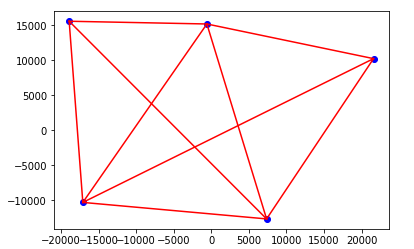
\includegraphics[scale=.5]{mesh.png}
	\caption{A mesh}
	\label{fig:mesh}
\end{figure}

Let us suppose one wants to solve such a problem on the mesh presented in figure \ref{fig:mesh}. Each node (blue) has un unknown potential $u$, and on each edge (red) there is an unknown oriented flux $f$. For each edge, there is also a given impedance $k$. On table \ref{tab:potNflux}, the physical quantities represented by $u$, $f$ and $k$ are listed.

\begin{table}[ht]
	\centering
	\begin{tabular}{ccccc}
      \toprule
		Domain & $u$ & $f$ & k & Remark \\
      \midrule
		Economy & Quantity of goods & Flux of goods & ? & \\
		Traffic modelling & Population & Traffic & ? & It's our case \\
		Thermic & Temperature & Heat flux & Thermal conductivity & \\
		Diffusion & Quantity of particles & Flux of particles & Conductivity & \\
		Electricity & Electric potential & Intensity & Inverse of resistance & \\
		Mechanics & Displacement & Stress & Stiffness & $u$ is a vector \\
      \bottomrule
	\end{tabular}
	\caption{Potential and Flux in different domains}
	\label{tab:potNflux}
\end{table}

One can impose three types of boundary conditions:

\begin{itemize}
	\item Dirichlet BC consist at imposing some values of $u$ at some nodes.
	\item Neumann BC consist at imposing an input flux $b$ at some nodes. This leads to $\sum_j f_j = b$ for all edges that start from the given node.
	\item Robin BC consist at imposing a linear relation between $u$ and $b$ at some node. This leads to $\sum_j f_j = \mu u$.
\end{itemize}

%\begin{table}[ht]
%	\centering
%	\begin{tabular}{|c|c|c|c|} \hline
%		Domain & Dirichlet & Neumann & Robin \\ \hline
%		Economy & ? & Someone produces a given quantity  & Someone adapts the production to demand \\
%		& & of goods per day & $\mu$ is linked to the price the factory wants to sell its goods \\ \hline
%		Traffic modelling & The nb of people in a room is given & ? & People want to leave (or go to) a place\\
%		& & & $\mu$ is linked to the space in the place \\ \hline
%		Thermic & Temperature is imposed & A heat flux is imposed & Thermal conductivity \\ \hline
%		Diffusion & Quantity of particles & Flux of particles & Conductivity \\ \hline
%		Electricity & Electric potential & Intensity & Inverse of resistance \\ \hline
%		Mechanics & Displacement & Stress & Stiffness \\ \hline
%	\end{tabular}
%	\caption{Physical meaning of different boundary conditions in different domains}
%	\label{tab:BC}
%\end{table}

Solving the impedance problem consists in determining the potential at each node and the flux at each edge of the graph from the given boundary conditions.

%\textit{Remark:} In the case where the discrete problem arises from the discretization of a PDE on a mesh, for example by the Finite Elements Method (which is not the case in this article), things are slightly different and for example the flux unknowns are stored at Gauss points.

\subsection{Numerical resolution of an impedance problem}

\subsubsection{Impedance matrix}

From the potentials $u_i$, one can build a vector $U$. This vector is the unknown of the problem, and the fluxes $f_j$ are computed by post processing $U$. For example, if the edge $j$ links the node $m$ to the node $n$, one has :

\begin{equation}\label{eqn:flux}
f_j = k_j(u_m-u_n)
\end{equation}

From the given impedances $k$, one can build an impedance matrix $K$, by assembly of elementary matrices $K_j^e$ build on each edge.

\begin{equation}
K_j^e = \begin{pmatrix} k_j & -k_j \\ -k_j & k_j \end{pmatrix}
\end{equation}

For example, on the given mesh of figure \ref{fig:mesh}, the impedance matrix would be :

\begin{equation}
K = \begin{pmatrix} k_1+k_2+k_3 & -k_1 & 0 & -k_2 & -k_3 \\
-k_1 & k_1+k_4+k_5+k_6 & -k_4 & -k_5 & -k_6 \\
0 & -k_4 & k_4+k_7+k_8 & -k_7 & -k_8 \\
-k_2 & -k_5 & -k_7 & k_2+k_5+k_7+k_9 & -k_9 \\
-k_3 & -k_6 & -k_8 & -k_9 & k_3+k_6+k_8+k_9 \end{pmatrix}
\end{equation}

This matrix is symmetric and the sum of coefficients on all lines and all columns is $0$. One can show that this matrix is also semi-definite positive. The kernel of this matrix is composed of uniform vectors on the connected parts of the graph, and there are as many zero eigenvalues as there are disconnected sub-graphs. This point is very important in our context as the universe of Naev composes a disconnected graph. For example, if we have a graph composed of $2$ disconnected regions, the eigenvectors will be :

\begin{equation}
V_1 = \begin{pmatrix} 1\\1\\1\\0\\0  \end{pmatrix}; \ \ V_2 = \begin{pmatrix} 0\\0\\0\\1\\1  \end{pmatrix}
\end{equation}

\subsubsection{Taking into account the boundary conditions}

There are 3 ways to take into account Dirichlet boundary conditions: penalization, substitution and Lagrange multipliers. All these operations lead to modifications of the matrix $K$ (and of the right hand side $B$). If there is at least one node with a Dirichlet BC on each connected part of the graph, the matrix $K$ becomes definite positive, which means that it has no more kernel and the linear system has a unique solution. In this report, we won't develop further on Dirichlet BCs

For Neumann BC, one assembles the right hand side $F$, that has the same size as $U$, and that concatenates the Neumann boundary conditions. The solution of the impedance problem is $U$ such that:

\begin{equation}
KU = F
\end{equation}

Robin boundary conditions are taken into account by adding $\mu$ to component $(i,i)$ of the matrix $K$, where $i$ is the index of the node where the Robin BC is applied. If there is at least one node with a Robin BC on each connected part of the graph, the matrix $K$ becomes definite positive, which means that it has no more kernel and the linear system has a unique solution.

\subsection{Impedance matrix kernel and resolution of the problem} \label{part:solve}

The kernel of the operator has a great importance as it makes the matrix singular, and consequently, it is not possible to solve straightforwardly a linear problem that implies this matrix. Actually, the solution of such a problem is not unique and any vector that is inside the kernel can be added to a solution.

Once one Robin BC has been added on each connected part of the graph, the system has an unique solution. This solution is also one of the solutions of the problem without the Robin BCs if there is only one Robin BC per connected part of the mesh, and if the right hand side is orthogonal to the kernel.

There are a few interesting properties that will be useful to determine automatically during computation if two nodes are connected by the graph:

\begin{itemize}
	\item If the right hand side is non-zero only in one connected sub-graph, the solution of the system vanishes in all the other sub-graphs.
	\item If the right hand side is orthogonal to the kernel of the matrix $K$ (ie. with zero mean), the solution at a node with Robin BCs is zero.
	\item If the right hand side is non-zero only in one connected sub-graph, and each of its terms is greater or equal to zero, the solution of the system vanishes only in the other sub-graphs, and is strictly greater than zero in the sub-graph.
\end{itemize}

By virtue of the last property, if the right hand side is $b_i = \delta_{ij}$ ($\delta$ being the Kronecker symbol, which means $0$ everywhere and $1$ on node $j$), the only nodes connected to $j$ are such that the corresponding component of $K^{-1}F$ is nonzero.

\subsection{Large sparse impedance problems}

In practice, when the problem get larger, each node tends to be linked to only a small part of all the other nodes. As a consequence, the matrix $K$ has many zero components. We refer at such a matrix as sparse. Performing linear algebra operations for sparse matrices is mathematically equivalent to performing the same operations on full matrices, but the computational cost can be vastly reduced if a spasre linear algebra library is used.

\section{Topological optimization problem}

The problem we are interested in consists in designing the best graph of lanes in some sense, given by a cost-function. In our application, the connectivity of the graph does not change during the optimization process. What changes is the impedance of each edge of the graph, that is influenced by the presence of a safe lane.

A node is created for each inhabited asset of each system, as well as for each jump point, and internal edges are considered between each couple of nodes in the same system. The impedance of an internal edge is taken as equal to the invert of its length, and is changed when a safe lane is activated. External edges are considered between jump points of different systems, and their impedance is fixed. This creates a sparse graph that links the assets. A few edges are then suppressed in case they are too close from an other shorter edge.

\subsection{Parameter-dependant impedance}

We denote by $L_j\in\mathbb{R}^*_+$ the length of an edge and $\theta_j^k\in\{0,1\}$ is $1$ if there is a safe lane of faction $k$ and $0$ otherwise. $\sum_k\alpha\theta_j^k$ can not be greater than $1$, which means that there can't be more than one lane per edge. $\alpha$ is the performance parameter of safe lanes. Here is how the impedance of an internal edge is computed :

\begin{equation}\label{eqn:stiff}
k_j = \dfrac{1+\sum_k\alpha\theta_j^k}{L_j}
\end{equation}

\textit{Remark}: For now, it is assumed that the impedance is the same for all factions, which is wrong at least in the case where these factions are enemies. Removing this hypothesis would mean that there is one impedance matrix per faction, and so one direct and adjoint problem per faction. This can be done, but will definitely have a big computational cost.

One finally ends up with an impedance matrix that is dependant on the set of parameters $\theta$, and that will from now be denoted by $K(\theta)$.

\subsection{Boundary conditions of the direct problem}

We choose to add a Robin boundary condition on an arbitrary node in each connected part of the graph. We refer as such nodes as anchors. If there is only one anchor per connected pert of the graph, and if the right-hand side is orthogonal to the kernel of $K$, one can show that the choice of the particular node has no impact on the solution of the problem.

If one wants to compute the path between two nodes, one has to put a Neumann condition of $1$ on the first node and $-1$ on the second node. The result is the flux of travellers when people want to go from one node to the other one.

The resolution of the entire impedance problem requests to solve the previous problem for any couple of assets, which would mean to solve and store the solution for $n(n-1)/2$ linear problems, where $n$ is the number of inhabited assets. This could lead to cause severe performance issues. However, thanks to the property of linearity of this problem, one can store only the $n$ solutions to problems with a Neumann condition on one node. This set of solutions is stored as a full matrix $\tilde{U}$ for which every column is the solution of one of these problems.

We introduce $\tilde{F}$, the multiple right hand side associated to the previous Neumann problems, and we get:

\begin{equation}
K(\theta)\tilde{U} = \tilde{F}
\end{equation}

If we introduce the multi-index $\eta = (i,j)$, one can also write the following relation:

\begin{equation}
f_{k,\eta} = \tilde{f}_{k,i} - \tilde{f}_{k,j},\ \ \forall k
\end{equation}

In a matricial notation, this writes :

\begin{equation}
F = \tilde{F} P^T
\end{equation}

Where $P$ is a sparse matrix of size $n(n-1)/2\times n$. This matrix can be assembled thanks to its sparsity. By linearity, one has also:

\begin{equation}
U = \tilde{U} P^T
\end{equation}

If $i$ and $j$ are not connected by the studied graph, which can be detected using the properties of part \ref{part:solve}, then the couple $(i,j)$ should not be considered in $P$. The corresponding line should be removed.

\subsection{Topological optimization procedure}

The principle of a topological optimization procedure is to build a cost-function $\phi(\theta)$ and find the best values of $\theta$ for which $\phi$ is minimal. One can introduce a function $\varphi(U,\theta)$ such that :

\begin{equation}
\phi(\theta) = \varphi(U,\theta),\ \text{with}\ K(\theta)U = F
\end{equation}

The sketch of the optimization process is as follows :

\begin{itemize}
	\item Initialization: $\theta_0$ is zero except for the lanes that are imposed as active
	\item At each iteration, compute $U$ by solving the multiple right hand side linear system $K(\theta_i)U=F$
	\item Find the next iterate $\theta_{i+1}$
\end{itemize}


\section{Cost-function and gradients}

\subsection{Minimization problem}

The cost-function should measure how hard it is to travel along the graph. It will be computed from the sum on all edges of the flux on this particular edge by the invert of the edge's impedance. On a given edge, one introduce $g_{j,\eta} = f_{j,\eta}/k_j$. One then has, according to \eqref{eqn:flux} the following result:

\begin{equation}
g_{j,\eta} = u_{m,\eta}-u_{n,\eta}
\end{equation}

This means that in our particular application, the cost-function $\varphi$ does not depend on $\theta$ directly. In a matricial notation, we introduce the sparse difference matrix $Q$ of size $n_{edges}\times n_{nodes}$:

\begin{equation}
G = QU = Q\tilde{U}P^T
\end{equation}

We introduce now the fact that there are different faction, each of them has its own weight for a given couple of nodes. This is taken into account with the diagonal weighting matrix $D_p$:

\begin{equation}
G_p = Q\tilde{U}P^TD_p
\end{equation}

One introduces $P_p = D_pP$, and then we have :

\begin{equation}
G_p = Q\tilde{U}P_p^T
\end{equation}

With this notation, $U$, which size is too big, has been replaced by $\tilde{U}$, but for clarity, we will still write $\varphi(\tilde{U})$. This cost-function itself is computed as the Frobenius norm of the matrix $G$, that is:

\begin{equation}\label{eqn:phi}
\varphi(\tilde{U}) = \dfrac{1}{2} \|Q\tilde{U}P_p^T\|_f^2
\end{equation}

Where :

\begin{equation}
\|G\|_f = \left(\sum_{i,j}g_{ij}^2\right)^{1/2}
\end{equation}

The minimization problem then reads:

\begin{equation}
\min_{K(\theta)\tilde{U} = \tilde{F}} \dfrac{1}{2} \|Q\tilde{U}P_p^T\|_f^2
\end{equation}

\subsection{The adjoint method}

Let us introduce the matrix term to term product: $c = A\cdot B$ means $\forall (i,j), c = \sum_{i,j} a_{ij} b_{ij}$.

In this part, we seek to determine the gradient of the cost-function $\phi$ with respect to $\theta$. In order to take into account the constraint $K(\theta)\tilde{U} = \tilde{F}$, one introduces the Lagrange multiplier $\Lambda$ and the Lagrangian $\psi(\theta,\tilde{U},\Lambda)$:

\begin{equation}
\psi(\theta,\tilde{U},\Lambda) = \dfrac{1}{2} \|Q\tilde{U}P_p^T\|_f^2 + \Lambda^T \cdot \left( K(\theta)\tilde{U} - \tilde{F} \right)
\end{equation}

One can show that the solution of the minimization problem is also the saddle-point of $\psi$. One can compute the gradients of $\psi$:

\begin{equation}
\begin{cases}
\nabla_u \psi = Q^TQ\tilde{U}P_p^TP_p + K(\theta)^T \Lambda \\
\nabla_\lambda \psi = K(\theta)\tilde{U} - \tilde{F} \\
\nabla_\theta \psi = \Lambda^T \cdot \nabla K(\theta) \tilde{U}
\end{cases}
\end{equation}

See annex A for the computation of $\nabla_u \psi$. The computation of $\nabla_\lambda \psi$ is not classic either, but quite straightforward.

For $\tilde{U}$ and $\lambda$ such that $\nabla_u \psi = 0$ and $\nabla_\lambda \psi = 0$, one has $\nabla\phi = \nabla_\theta \psi$.

\textit{Remark:} As $\nabla K$ is symmetric, one can show that $\Lambda^T \cdot \nabla K(\theta) \tilde{U} = \tilde{U}^T \cdot \nabla K(\theta) \Lambda$

As a conclusion, in order to compute $\nabla\phi$, which is an essential point in the algorithm, one has to do the following computations :

\begin{itemize}
	\item Solve MRHS problem $K(\theta)\tilde{U} = \tilde{F}$ to obtain $\tilde{U}$
	\item Solve MRHS problem $K(\theta) \tilde{\Lambda} = - Q^TQ\tilde{U}$ to obtain $\tilde{\Lambda}$
	\item Compute $\Lambda = \tilde{\Lambda}P_p^TP_p$
	\item Evaluate $\nabla\phi = \Lambda^T \cdot \nabla K(\theta) \tilde{U}$, as detailed in annex C.
\end{itemize}

\section{The algorithm (boolean case)}

We propose first an algorithm that works with boolean unknowns $\theta$. It consists in activating at each iteration one lane per system and per faction. This lane is the one with the strongest gradient (in absolute value). It is presented at algorithm \ref{alg:lanes}.

\begin{algorithm}[ht]
	\caption{Lanes building algorithm}
	\label{alg:lanes}
	\begin{algorithmic}
		\STATE Compute $Q$ and $Q^TQ$
		\STATE For each faction, compute $P_p$ and $P_p^TP_p$
		\STATE Assemble the MRHS $\tilde{F}$
		\STATE Initialize the vector $\theta_1$
		\FOR{$i = 1,\,2,\, \dots,n$}
			\STATE Compute $K(\theta_i)$
			\STATE Solve $K(\theta_i)\tilde{U} = \tilde{F}$
			\STATE Solve $K(\theta_i)\tilde{\Lambda} = - Q^TQ\tilde{U}$
			\STATE For each faction, compute $\Lambda_p = \tilde{\Lambda}P_p^TP_p$
			\STATE Compute for each faction $\nabla\phi = \Lambda_p^T \cdot \nabla K(\theta) \tilde{U} = \left( ( \Lambda_p\tilde{U}^T )_{ii} + ( \Lambda_p\tilde{U}^T )_{jj} - ( \Lambda_p\tilde{U}^T )_{ij} - ( \Lambda_p\tilde{U}^T )_{ji} \right) k_{ij}$
			\FOR{Each system $s$}
				\FOR{Each faction $p$}
					\STATE Activate the affordable lane for which the ratio $\nabla\phi_\eta / L_\eta$ is the greatest.
				\ENDFOR
			\ENDFOR
		\ENDFOR
	\end{algorithmic}
\end{algorithm}

\section{Continuous case}

In the case where $\theta$ represents the density of a given lane, on which the only constraint is that it is positive, a steepest-descent algorithm can be proposed.

\textcolor{red}{Watch out: this part is a draft}

\textcolor{red}{It might be interesting to precondition the algo by multiplying the gradient by the invert of the lengths of the lanes, as done in the boolean case. OR not}

\subsection{Constrained optimization}

\subsubsection{Lanes costs}

For each system, and each faction, the total cost of lanes must be equal to the faction's presence in the system, which can be represented as the following constraint, where $\xi_j$ is the cost of a given lane, and $\Xi_p$ is the presence of the faction $p$:

\begin{equation}
\forall s \text{ (system)}, \forall p \text{ (faction)}, \sum_j \theta_j^p \xi_j = \Xi_p
\end{equation}

This can be enforced by initializing $\theta$ for each system and faction as:

\begin{equation}
\forall s \text{ (system)}, \forall p \text{ (faction)}, \forall j \text{ (lane)}, \theta_{j,0}^p = \dfrac{\Xi_p}{\sum_i \xi_i}
\end{equation}

And by enforcing that, for any update $\delta$:

\begin{equation}
\forall s \text{ (system)}, \forall p \text{ (faction)}, \sum_j \delta_j^p \xi_j = 0
\end{equation}

Two different cases may happend:

1/ There is only one lane in the system: $\delta_0^p = 0$ all the time for any faction

2/ There is more than one lane: one can select one lane (for example the last one in the list), which density will automatically determined from the density of the other lanes:

\begin{equation}
\forall s \text{ (system)}, \forall p \text{ (faction)}, \delta_{end}^p = - \dfrac{1}{\xi_{end}} \sum_j \delta_j^p \xi_j
\end{equation}

This second point leads to a variable change that can be formally written as follows, where $c$ is a vector for each system and faction:

\begin{equation}
\theta_{end} = c^T \theta_0
\end{equation}

We define the cost-function, depending only on $\theta_0$:

\begin{equation}
\tilde{\phi}(\theta_0) = \phi(\theta_0,c^T\theta_0)
\end{equation}

Its gradient is then \textcolor{red}{CHECK THIS ONE}:

\begin{equation}
\nabla\tilde{\phi}(\theta_0) = \nabla_{\theta_0}\phi(\theta_0,c^T\theta_0) + c^T\nabla_{\theta_{end}}\phi(\theta_0,c^T\theta_0)
\end{equation}

\subsubsection{Positivity of density} \label{sect:pos}

The second constraint is the positivity of the lane density. This reads $\theta\geqslant0$. With the previous variable change, it reads rather:

\begin{equation}
\begin{cases}
	\theta_0 \geqslant 0\\
	c^T\theta_0 \geqslant \Xi
\end{cases}
\end{equation}

\textcolor{red}{Check the second inequality}

From any tentative iterate $\tilde{\theta_0}$, the vector $\theta_0$ will be constructed by projection:

\begin{equation}
\theta_0 = \argmin_{\substack{\theta \geqslant 0\\c^T\theta \geqslant \Xi}} \dfrac{1}{2}\|\theta-\tilde{\theta_0}\|^2
\end{equation}

\textcolor{red}{TODO: it might be interesting to add a term $1/2 c^T(\theta-\theta_0)$ to make the result independent of the choice of $\theta_{end}$, but it makes the problem more complicated}

The projection can be performed independently in each system and for each faction.

\subsection{Linesearch step}

The gradient gives the direction to follow for minimizing $\theta$. Once this direction $\delta$ is known, one has to solve the 1-D minimization problem by dichotomy. We define two candidates next iterates: $\alpha$ and $\beta$, and an initial step $p$. They will converge towards the optimal point.

The operation of projection presented in Section~\ref{sect:pos}, will be denoted by $P(\bullet)$

\begin{algorithm}[ht]
	\caption{Linesearch}
	\label{alg:linesearch}
	\begin{algorithmic}
		\STATE Initialize $\alpha = \theta_n$, the previous iterate.
		\STATE Initialize $\beta = \alpha + p\delta$
		\IF{$\phi(P(\alpha))>\phi(P(\beta))$}
		\STATE $\gamma\leftarrow \dfrac{-\alpha+2\beta}{2}$
		\WHILE{$\phi(P(\beta))>\phi(P(\gamma))$}
		\STATE $\beta\leftarrow\gamma$
		\STATE $\gamma\leftarrow \dfrac{-\alpha+2\beta}{2}$
		\ENDWHILE
		\ENDIF
		\STATE \COMMENT{Now, we know there is a minimum between $\alpha$ and $\beta$}
		\FOR{Each $i=1..n$}
		\IF{$\phi(P(\alpha))>\phi(P(\beta))$}
		\STATE $\alpha\leftarrow \dfrac{\alpha+\beta}{2}$
		\ELSE
		\STATE $\beta\leftarrow \dfrac{\alpha+\beta}{2}$
		\ENDIF
		\ENDFOR
		\STATE $\theta_{n+1} = P(\alpha)$
	\end{algorithmic}
\end{algorithm}

\textcolor{red}{Check the algo}

\subsection{Evaluation of the cost-function}

\textcolor{red}{Abuse of notation}

\begin{equation}
\phi(\theta) = \varphi(\tilde{U}(\theta)) = \dfrac{1}{2} \|Q\tilde{U}P_p^T\|_f^2
\end{equation}

\textcolor{red}{Each evaluation is very likely to be very costly. Try to find a trick, otherwise we're doomed.}

\subsection{Regularization}

In the case when the algorithm tends towards activating only one lane with its full presence, it might be interesting to regularize the solution by adding to the cost-function a term of the form:

\begin{equation}
N(\theta) = \dfrac{\mu}{2} \|\theta\|^2
\end{equation}

Of course, the weight $\mu$ is a new parameter of the method that has to be determined by hand (or maybe with a L-curve?)

\section{Conclusion}

In this report, an algorithm was presented, that aims at generating a mesh of safe lanes via the resolution of a topological optimization problem based on the impedance problem.

\section*{Annex A: computation of derivative for the Frobenius norm}

We develop the computation of $\nabla_u\varphi$

\begin{equation}
\varphi = \dfrac{1}{2} \sum_{i,l} \sum_{j,k} \left(q_{ij} \tilde{u}_{jk} p_{lk}\right)^2
\end{equation}

\begin{equation}
\nabla_u\varphi|_{mn} = \dfrac{\partial\varphi}{\partial u_{mn}} = \sum_{i,l} q_{im}p_{ln} \sum_{j,k} q_{ij} \tilde{u}_{jk} p_{lk}
\end{equation}

This leads to:

\begin{equation}
\nabla_u\varphi = Q^TQ\tilde{U}P^TP
\end{equation}

\section*{Annex B: Evaluation of the gradient}

We evaluate in this part $\nabla\phi = \Lambda^T \cdot \nabla K(\theta) \tilde{U}$. As $\nabla K(\theta)$ is an order $4$ tensor, (because $\theta$ is indexed by a multi-index), it is absolutely out of question to assemble it. For that reason, a smarter approach is needed.

We introduce $k_{ij} = \alpha/L_{ij}$, and the Kroneker symbol $\delta$. From \eqref{eqn:stiff}, one has:

\begin{equation}
\nabla K(\theta_{ij})|_{kl} = \delta_{ik} \delta_{il} k_{ij} + \delta_{jk} \delta_{jl} k_{ij} - \delta_{ik} \delta_{jl} k_{ij} - \delta_{jk} \delta_{il} k_{ij}
\end{equation}

\begin{equation}
\begin{aligned}
\left( K(\theta_{ij}) \tilde{U} \right)|_{km} &= \sum_l \left( \delta_{ik} \delta_{il} k_{ij} + \delta_{jk} \delta_{jl} k_{ij} - \delta_{ik} \delta_{jl} k_{ij} - \delta_{jk} \delta_{il} k_{ij} \right) u_{lm}\\
&= \delta_{ik} k_{ij} u_{im} + \delta_{jk} k_{ij} u_{jm} - \delta_{ik} k_{ij} u_{jm} - \delta_{jk} k_{ij} u_{im}
\end{aligned}
\end{equation}

\begin{equation}
\begin{aligned}
\nabla\phi|_\eta = \nabla\phi|_{ij} &= \sum_{k,m} \lambda_{km} \left( \delta_{ik} k_{ij} u_{im} + \delta_{jk} k_{ij} u_{jm} - \delta_{ik} k_{ij} u_{jm} - \delta_{jk} k_{ij} u_{im} \right)\\
&= \sum_m \left( \lambda_{im} k_{ij} u_{im} + \lambda_{jm} k_{ij} u_{jm} - \lambda_{im} k_{ij} u_{jm} - \lambda_{jm} k_{ij} u_{im} \right)\\
&= \left( ( \Lambda\tilde{U}^T )_{ii} + ( \Lambda\tilde{U}^T )_{jj} - ( \Lambda\tilde{U}^T )_{ij} - ( \Lambda\tilde{U}^T )_{ji} \right) k_{ij}
\end{aligned}
\end{equation}

\end{document}
